\documentclass{article}

\usepackage{Sweave}
\begin{document}
\Sconcordance{concordance:tobdel2.tex:tobdel2.Rnw:%
1 2 1 1 0 6 1 1 2 1 0 8 1 1 4 8 0 1 3 3 1 1 2 1 0 3 1 1 2 1 0 1 1 10 0 %
1 2 1 1 1 2 1 0 5 1 1 6 5 0 7 1 10 0 1 2 1 1 1 2 5 0 1 2}


\section{Prediction theory}
There is a growing interest in applying these models to clinical prediction and personalized medicine. The goal of these applications is that model based  predictions increase the chances of survival of the patients. Furthermore, these predictions become more accurate when more information becomes available. A typical application is to tailor the medical treatment based on the survival probabilities derived from our jointmodel, that is, to intervene when the medical prognosis deteriorates.

$$\beta$$ is my favourite section of the r language documentation.
\begin{Schunk}
\begin{Sinput}
> library(lme4)
> library(smoothLME)
> library(lattice)
> library(lcmm)
> data(Cholesterol, package = "qrLMM")
> Cholesterol$resp <- Cholesterol$cholst/100
> Cholesterol$time <- (Cholesterol$year - 5)/10
> Cholesterol.samp <- subset(Cholesterol, newid %in% 1:16)
> Cholesterol.samp$newid <- as.factor(Cholesterol.samp$newid)
> xyplot(cholst ~ year | newid, data = Cholesterol.samp,
+        type = c("p", "r"), lwd = 2, layout = c(4, 4),
+        as.table = TRUE, ylab = "Cholesterol", grid = TRUE,
+        xlab = "Time (years)")
> 
\end{Sinput}
\end{Schunk}
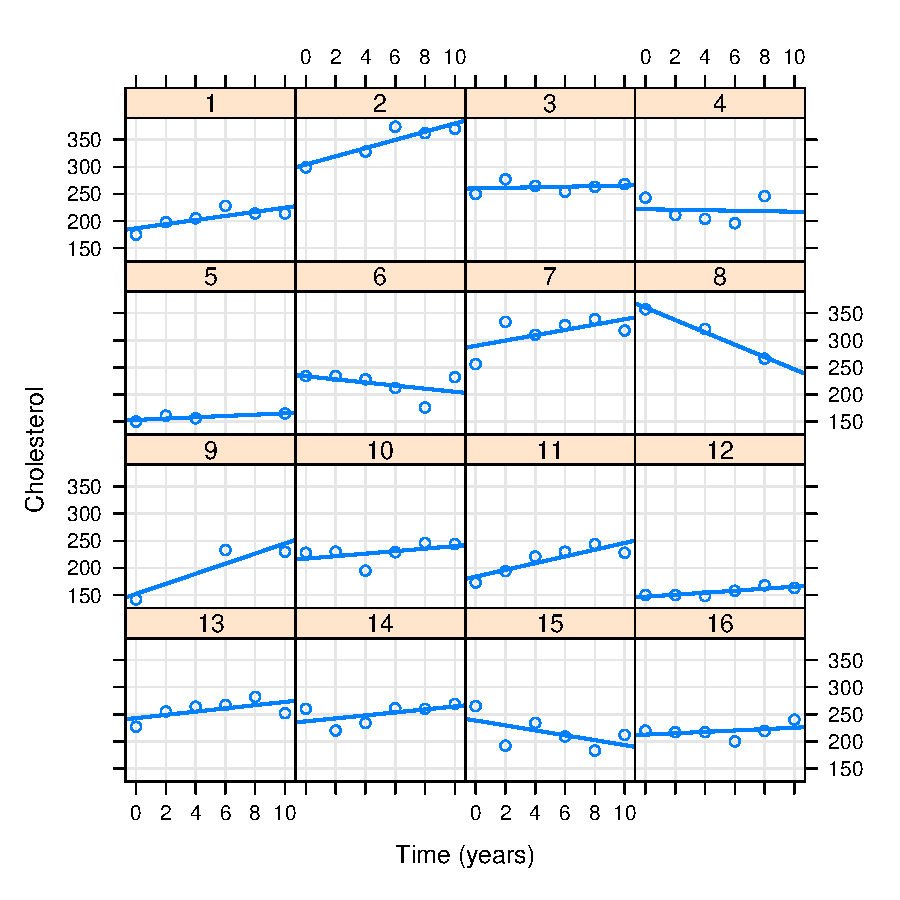
\includegraphics{tobdel2-001}

\section{Joint model}
We fit the joint model to the pbc data.

\begin{Schunk}
\begin{Sinput}
> library(smoothJM)
> data("pbc2", package = "JM")
> pbc2$lsgot <- log(pbc2$SGOT)
> pbc2$id <- as.numeric(pbc2$id)
> model1 <- smoothJM(lsgot ~ year +  (1 + year | id), maxiter = 250,
+ survival = Surv(years, status2) ~ factor(drug) + factor(sex), data = pbc2, n1 = 3, n2 = 3, rightskewed = c(T,T))
> model1$survmodel
\end{Sinput}
\begin{Soutput}
              coefficient        SE          z     p.value
drugD-penicil  0.03069024 0.1714289  0.1790261 0.857917216
sexfemale     -0.67415357 0.2195564 -3.0705258 0.002136822
bm_intercept   1.02607070 0.1213681  8.4542062 0.000000000
bm_slope       1.52222208 0.1292386 11.7783890 0.000000000
\end{Soutput}
\end{Schunk}
this is the end of the document and a test.
\section{Aids example}
\begin{Schunk}
\begin{Sinput}
> data(aids, package="JM")
> aids$CD4W <- sqrt(aids$CD4)
> aids$patient <- as.numeric(aids$patient)
> col_v <- vector(length=9)
> lty_v <- vector(length=9)
> c1 <- c("red","blue","black")
> for( i in 1:3){
+    for( j in 1:3){
+       col_v[(i-1)*3+j]<-c1[i]
+       lty_v[(i-1)*3+j]<-j
+    }
+ }
> examp <- smoothJM(CD4W~ obstime + (1+obstime|patient), survival = Surv(Time, death) ~ factor(drug) + factor(gender), data =  aids, n1 = 3, n2 = 3, maxiter = 125)
> oldpar <- par()
> par(mfrow=c(1,2))
> plotrandomeffects(examp, which = "intercept", xlab = "intercept")
> plotrandomeffects(examp, which = "slope", xlab = "slope")
> par(mfrow=oldpar$mfrow)
> examp$crosstable
\end{Sinput}
\begin{Soutput}
          [,1]       [,2]       [,3]
[1,] 0.2726611 0.12111436 0.05379824
[2,] 0.1958540 0.08699714 0.03864359
[3,] 0.1406831 0.06249055 0.02775791
\end{Soutput}
\end{Schunk}
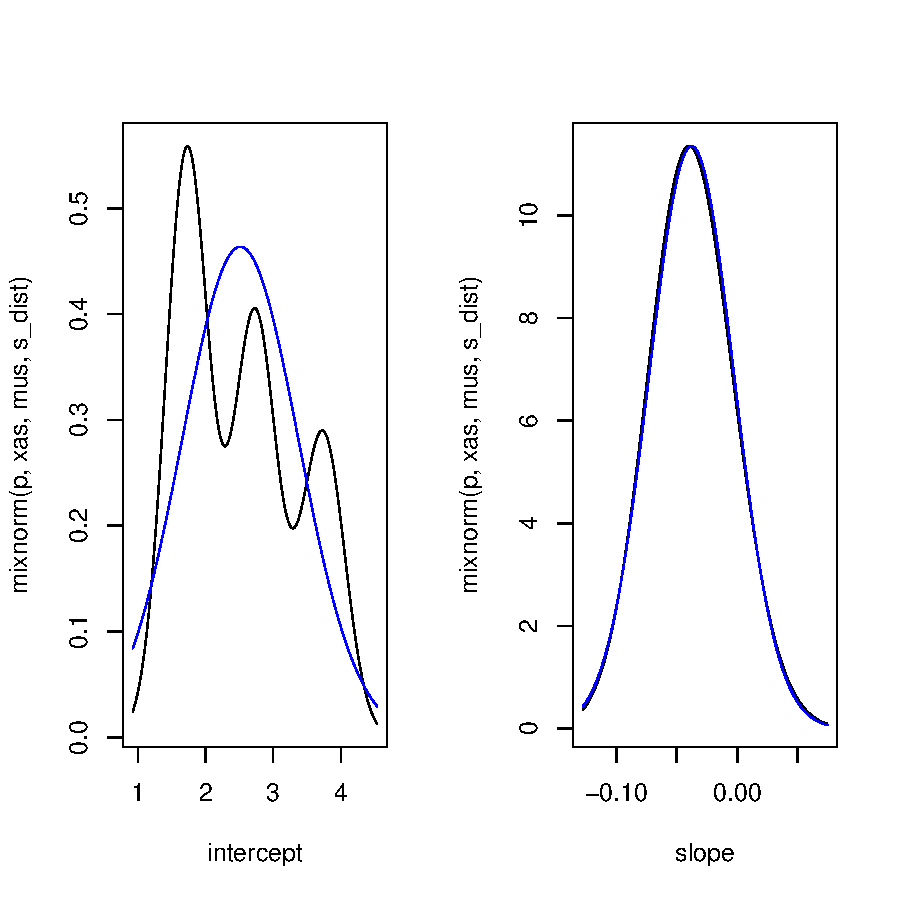
\includegraphics{tobdel2-003}

Survival plot
\begin{Schunk}
\begin{Sinput}
> plot(examp$jlcmm, which = 'survival',col = col_v,lty = lty_v, lwd = 2)
\end{Sinput}
\end{Schunk}
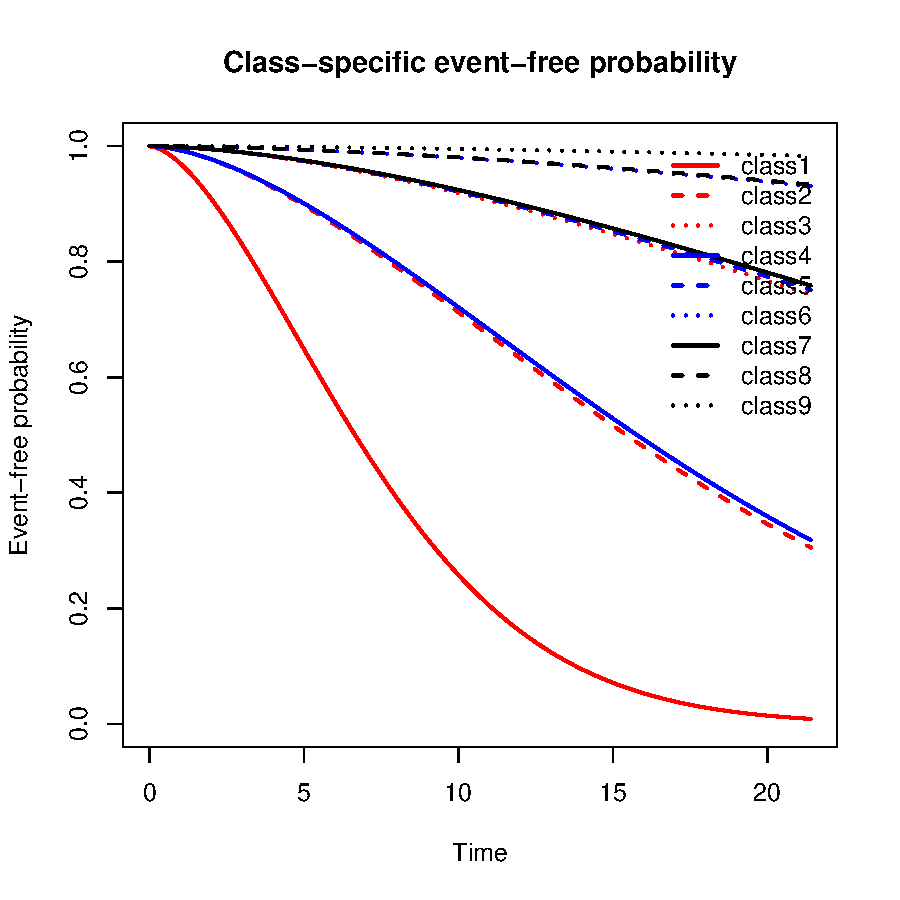
\includegraphics{tobdel2-004}
\end{document}
